\documentclass[11pt]{article}           % Set default font size, document style.

\usepackage[margin=1.2in]{geometry}     % Change margin sizes.
\usepackage{fancyhdr}                   % Modify page header/footer.
\usepackage[bookmarks, pdfauthor={Brian Kubisiak}]{hyperref}
\usepackage[parfill]{parskip}           % Paragraph style.
\usepackage{todonotes}                  % For adding TODO statements.
\usepackage[mode=text]{siunitx}         % Units. Use main font instead of math.
\usepackage{listings}                   % Listing source code
\usepackage{sourceserifpro}             % Main font.
\usepackage{sourcecodepro}              % Code font.
\usepackage{microtype}                  % Justify paragraphs a little better.

% set options for fancy header
\pagestyle{fancyplain}
\date{}
\setlength{\headheight}{18pt}

% code input
\lstset{basicstyle=\ttfamily\footnotesize, numbers=left, frame=single, tabsize=4}

\def\doctitle{EE 90 Project Documentation}
\hypersetup{pdftitle={\doctitle}}

% Add a title block.
\title{Smart Dog Bowl Using FFT Analysis of Dog's Bark}
\author{Brian Kubisiak \\ brian.kubisiak@gmail.com \\ MSC 606}

\begin{document}

\lhead{\large{Brian Kubisiak}}
\chead{\large{\doctitle}}
\rhead{\large{\today}}

\maketitle

\thispagestyle{empty}

\section{Motivation}
\label{sec:motivation}

In designing a smart dog bowl to open only for a specific dog, it is important
that method used for identifying the dog be very accurate; there should never be
a case where a dog is unable to access his food. Obvious approaches to this
problem would be to put some sort of identification tag on the dog's collar,
such as RFID or a modulated IR beacon.

However, these approaches can easily break down under fairly common
circumstances---IR must have a clear path to the sensor, and RFID depends on a
specific orientation. In addition, these approaches require the dog to be
wearing his collar, and---in the case of IR---the collar must be powered. I
believe that the most important part of this bowl is that a dog must never
approach his bowl, only to have it not open due to something blocking the
identification on his collar.

\section{Method of Approach}
\label{sec:method_of_approach}

To solve the problems described above, I have elected to identify the dog using
its bark. Just as humans each have a distinct-sounding voice, a dog's bark
contains a unique spectrum of frequencies. By analyzing these frequencies, I
believe that a system can be designed that will open for one dog's bark but not
another's.

The dog can never really ``lose'' his bark, so it is ideal in that the dog will
always be able to open the dish on his own. Additionally, in the case that an
error causes the dog to be misidentified, the dog will likely try again,
reducing the probability of error.

One disadvantage of this design is that the dog will have to be trained to bark
in order to open his food dish. However, this seems fairly easy, as teaching a
dog to ``speak'' is a fairly common trick. Another obvious disadvantage is that
the analysis will not get a distance measurement to the dog. In order to
overcome this, I will use ultrasonic ranging sensors to determine whether or not
the dog is within a \SI{1}{ft} radius.

\section{Hardware Operation}
\label{sec:operation}

My design comprises a microphone with an audio amplifier, triggering logic for
generating interrupts, ultrasonic rangefinders for measuring proximity, an
Arduino for performing the signal processing, and a servo motor for opening the
dog bowl.

All of the signal processing for this design will be performed on an Arduino
board. The processor will sample the dog's bark, then perform an FFT on the data
and compare it to saved values. If the bark matches, the bowl will open.

There will be 4 ultrasonic proximity detectors to determine whether or not there
is an object within \SI{1}{ft} of the bowl. This will consist of an ultrasonic
range finder and circuitry comparing it to a reference range. This detector will
output a digital 1 if there is an object within a foot, and a 0 if there is not.
Each range finder can detect in a \SI{15}{\degree} angle. By putting 4 of these
in a circle around the bowl, they should be able to detect anything larger than
a foot wide around the entire radius. More sensors can easily be used, at a
slightly increased cost.

The microphone will output a simple analog signal into the Arduino. In addition,
some analog circuitry will be used to generate an interrupt whenever the analog
input reaches a certain threshold in order to allow the Arduino to idle at lower
power when data is not being read.

A block diagram for this design is shown in figure (\ref{fig:diagram}).

\begin{figure}[h]
    \centering
    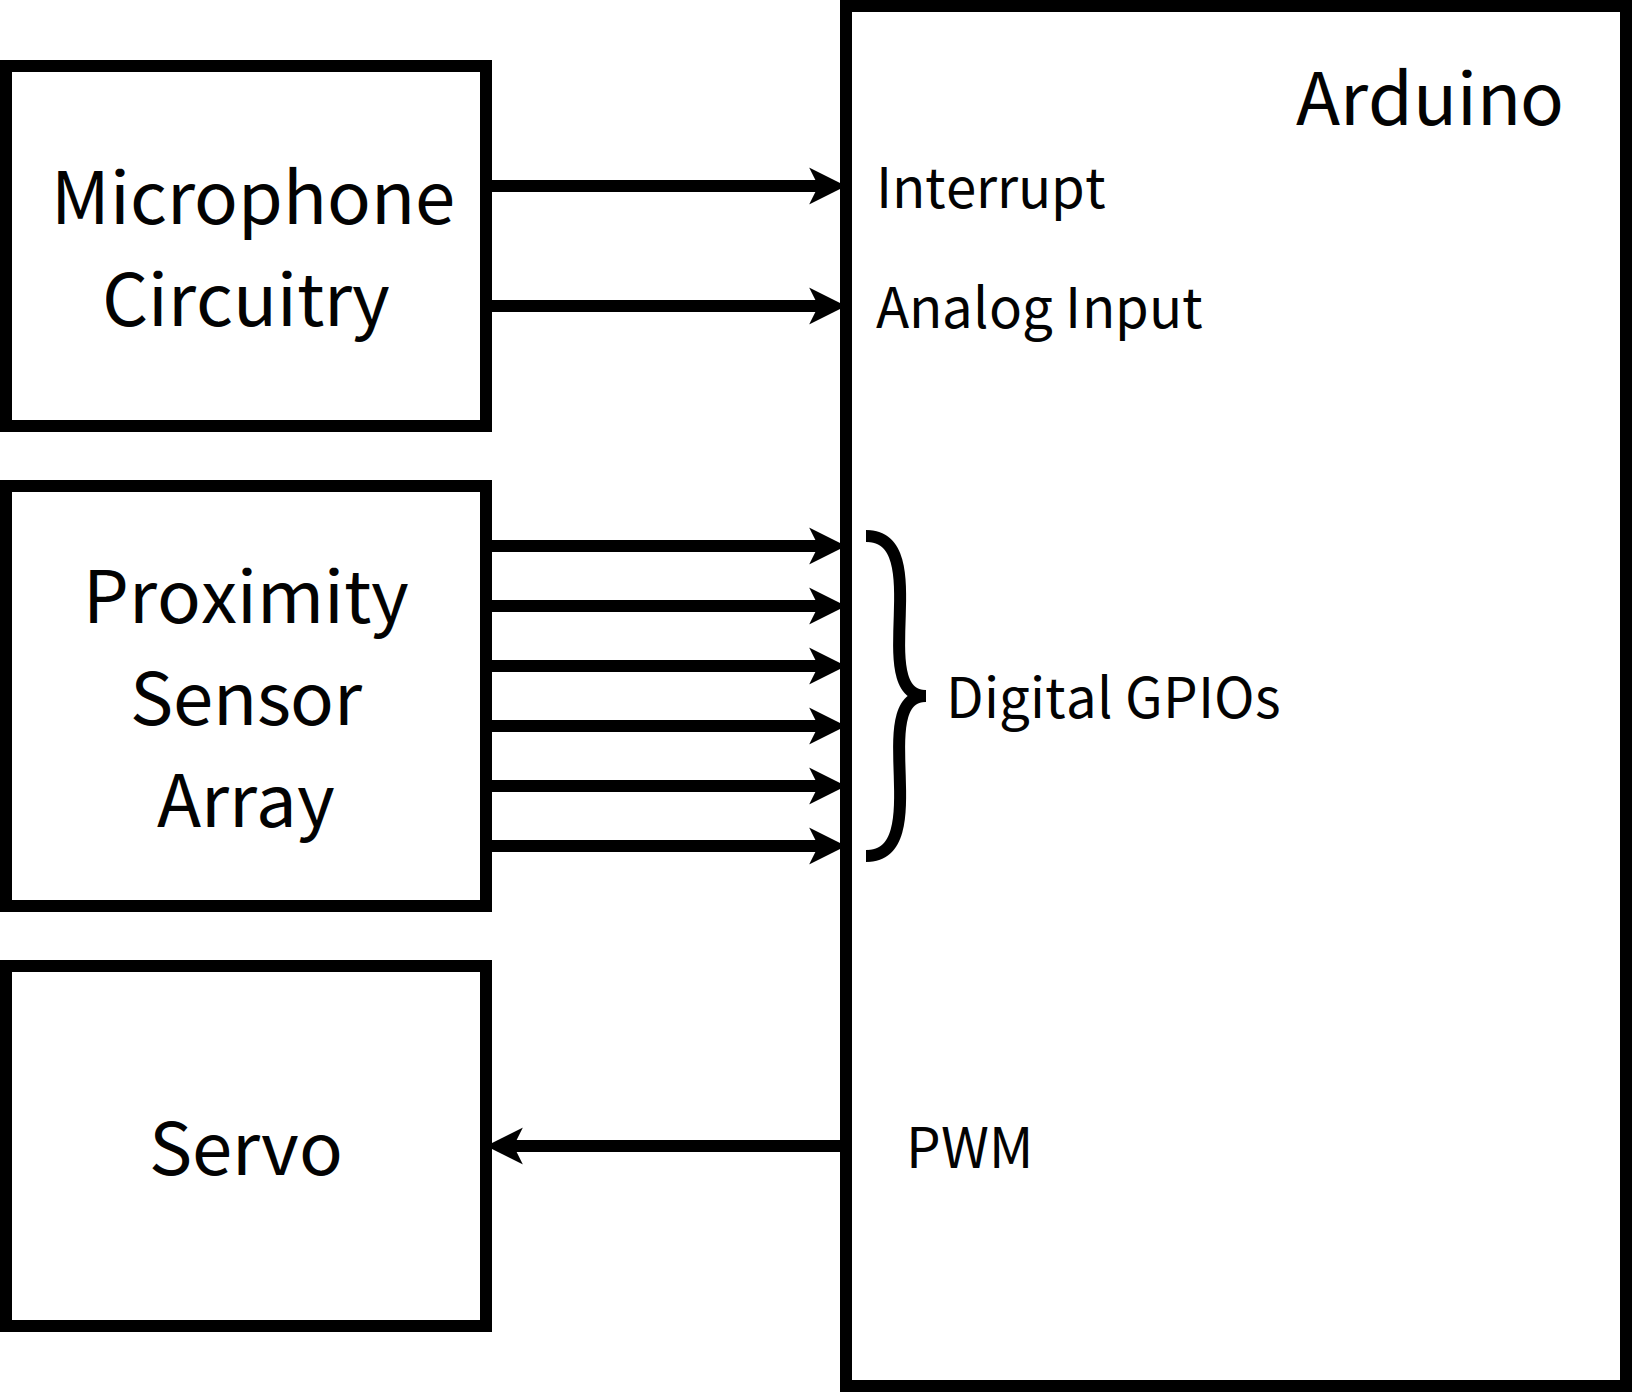
\includegraphics[width=0.4\linewidth]{sch/top-level.png}
    \caption{Top-level block diagram for the dog bowl.}
\label{fig:diagram}
\end{figure}

\subsection{Microphone Circuitry}
\label{sub:microphone_circuitry}

All of the microphone circuitry is detailed in figure~(\ref{fig:microphone}).

The microphone is powered from Vcc through a \SI{2.2}{\kilo\ohm} resistor,
as recommended in the data sheet. The signal is then lowpass-filtered before
being fed into the amplifier. The lowpass filter is designed with a corner
frequency of \SI{10}{\hertz} using R2 = \SI{100}{\kilo\ohm} and C1 =
\SI{1}{\micro\farad}. This will filter out the DC component without affecting
the AC signal.

The audio amplifier uses an op-amp with a single-sided supply in order to
amplify the input signal. The amplifier is arranged in a noninverting
configuration, with a total amplification factor of 560 (\SI{27.5}{\deci\bel}).
The resistor Rf can be adjusted as needed to change the amplification. Note
that the AC input may go below ground, but this will be clipped by the
amplifier.

The output of the amplifier is then fed directly into the ADC on the Arduino
board. This amplified signal is also fed into the comparator U2 in order to
generate an interrupt to tell the Arduino to begin recording the audio. The
trigger level is set with R4 and R5. I have found that a level of around
\SI{1.7}{\volt} works well. This interrupt trigger is fed into a GPIO pin on the
Arduino to generate an interrupt.

\begin{figure}[h]
    \centering
    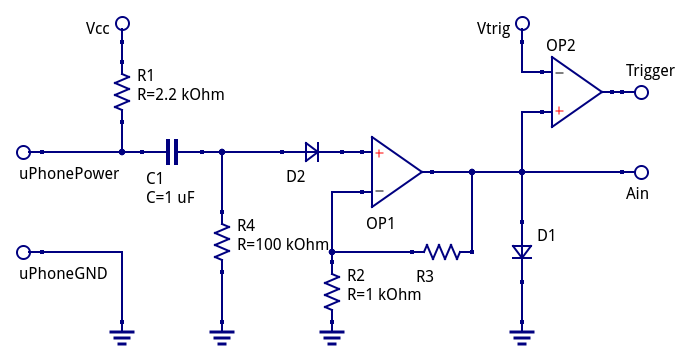
\includegraphics[width=0.8\linewidth]{sch/microphone.png}
    \caption{Microphone amplifier and trigger generator.}
\label{fig:microphone}
\end{figure}

\subsection{Proximity Sensor Array}
\label{sub:proximity_sensor_array}

The proximity sensor array is shown in figure~(\ref{fig:rangefinders}).

The sensor array is fed by ultrasonic range finders. Each range finder outputs
an analog voltage representing the distance to the nearest object (the exact
relation is not important to this design). The output of these sensors will be
fed into comparators, comparing them to a fixed voltage. This voltage will
correspond to approximately \SI{1}{ft} from the ultrasonic sensors. The voltage
is created using a voltage divider with the resistors R6 and R7. I have found
that a voltage level of \SI{0.76}{\volt} works well for identifying objects
approximately \SI{1}{ft} away.

The outputs from all of these comparators will go into GPIO pins on the Arduino.
When the microphone circuit triggers a recording, the Arduino will first check
that at least one of the proximity sensors is triggered before computing the
FFT of the recording.

Note that the comparators used in my design are open drain, so they do not drive
the output to Vcc; rather, they put the output in a high-impedance state that
requires a pull-up resistor. The Arduino GPIO pins have internal pull-up
resistors, so these are not included in my analog circuitry.

\begin{figure}[h]
    \centering
    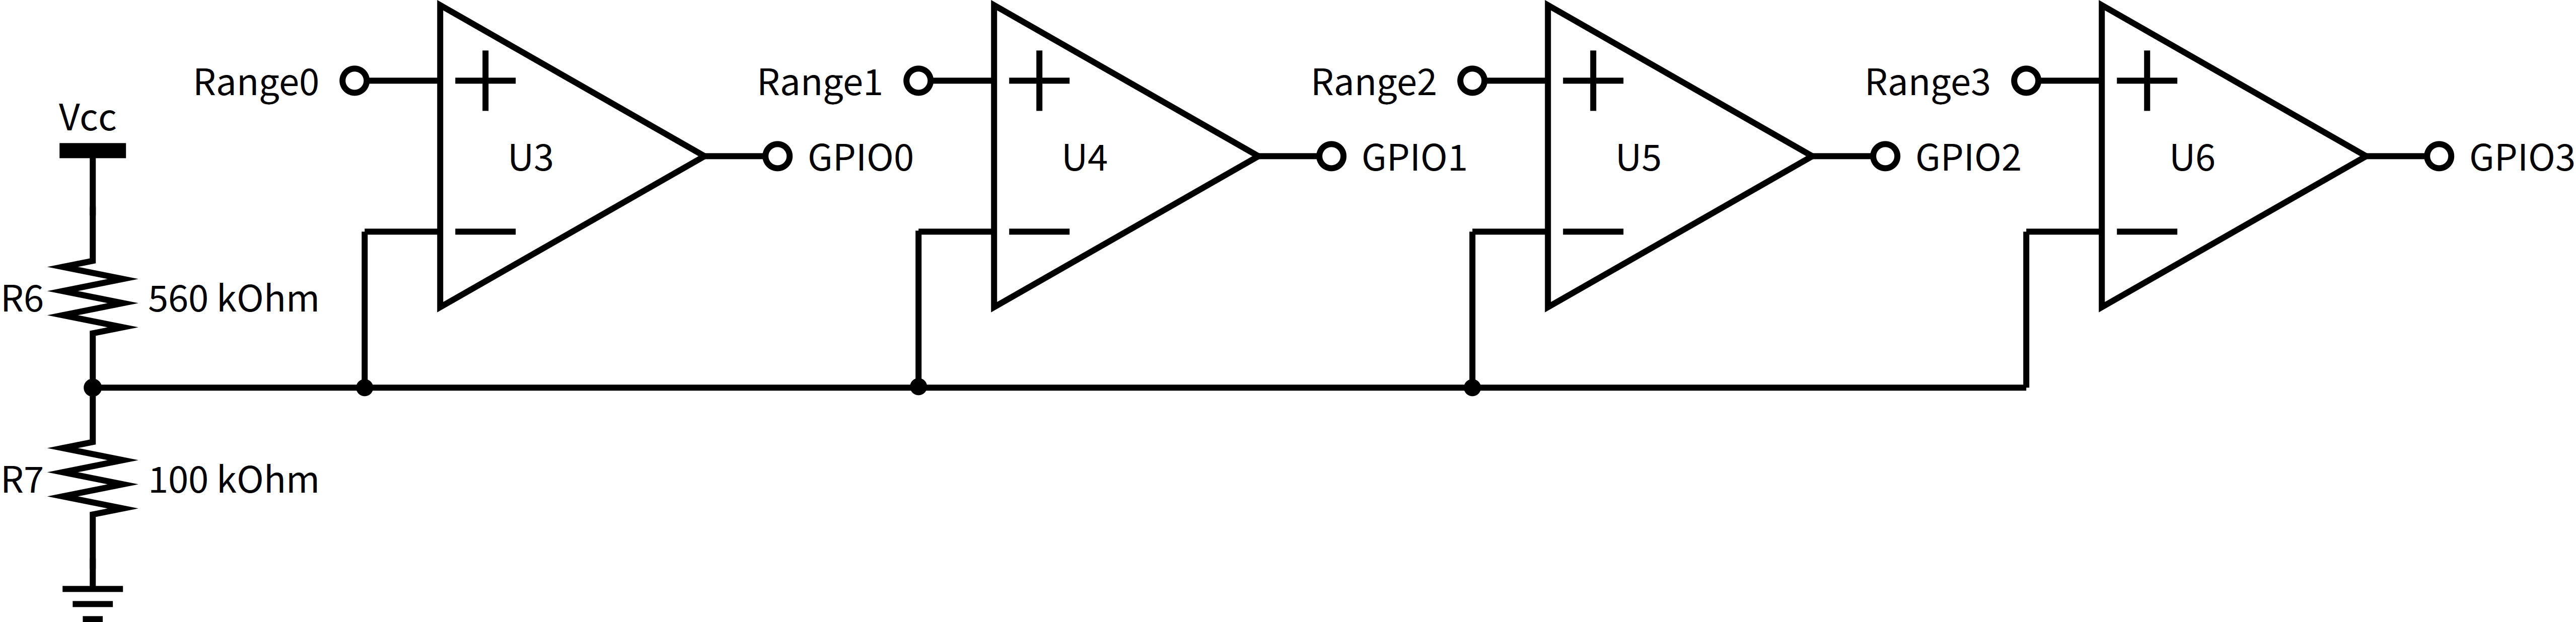
\includegraphics[width=1.0\linewidth]{sch/rangefinders.png}
    \caption{Circuit for the array of proximity sensors.}
\label{fig:rangefinders}
\end{figure}

\subsection{Servo Motor}
\label{sub:servo_motor}

The servo motor is a standard Parallax servo motor with \SI{180}{\degree} of
motion. The position of the servo is controlled through PWM\@. One of the PWM
outputs on the Arduino will switch the servo between the open position and the
closed position when needed.

\section{Software Operation}
\label{sec:source_code_listing}

The main loop for the software is a simple finite state machine, shown in
figure~(\ref{fig:fsm}). The machine starts in the INIT state. Once data is
available to analyze, the program checks if there is anything in the proximity
of the bowl. If there is, then the FFT analysis is performed. If not, the data
collection is reset.

If the FFT analysis finds that the frequency spectrum matches the spectrum of
the key, then the bowl is opened. Otherwise, the data collection is reset. Once
the bowl is open, it will just wait until nothing is nearby (i.e.\ the proximity
sensors are no longer activated). At this point, the bowl will be reset.

\begin{figure}[h]
    \centering
    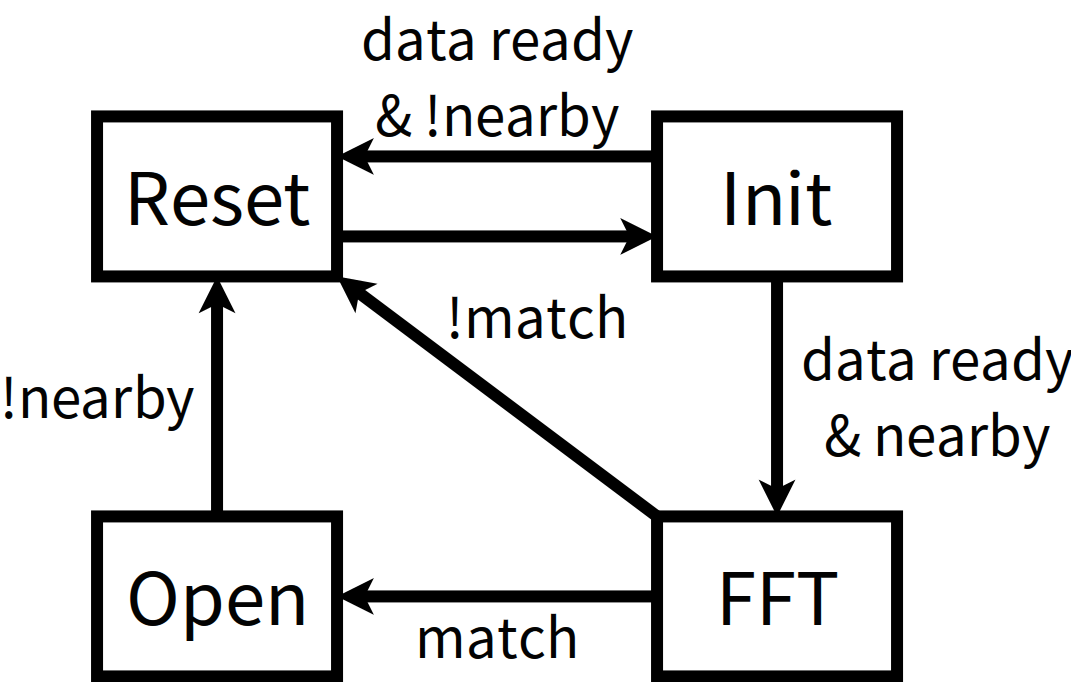
\includegraphics[width=0.4\linewidth]{sch/fsm.png}
    \caption{Finite state machine for controlling the dogbowl.}
\label{fig:fsm}
\end{figure}

\section{Results}
\label{sec:results}

The end result of my design is moderately successful. The Fourier analysis will
usually trigger after a few seconds of barking, and is unlikely to get a false
positive. This project is a good proof-of-concept, and I believe with a few
improvements, it would work fairly reliably.

The first improvement I would make would be to use a DSP for the signal
processing; with a more powerful chip, my project could perform a larger FFT and
more sophisticated error analysis. Additionally, adding a faster ADC would allow
me to sample the full audible frequency spectrum. This would likely reduce the
false positives by comparing a wider spectrum of frequencies.

Another limitation I encountered is that my microphone is poorly placed in the
final design. When I was constructing the circuit, I did not consider how the
whole design would be assembled and packaged. As a result, the microphone ended
up in a place that did not get a clear audio signal. The most important lesson
that I have learned from this project is to always think about the final
packaging and design so that choices made at the beginning do not limit the
design later.

The last problem I had with my design is that the ultrasonic sensors should be
angled upwards at a steeper angle. As they are now, they can be triggered by the
floor. This is an issue because the bowl will remain open even after the dog has
left. Again, anticipating the final design would have allowed me to fix this.

\section{Source Code Listing}
\label{sec:source_code_listing}

\subsection{Analog Data Collection Function Declarations}
\label{sub:data_collection_function_declarations}

\lstinputlisting{src/adc.h}

\subsection{Analog Data Collection Functions}
\label{sub:analog_data_collection_functions}

\lstinputlisting{src/adc.c}

\subsection{Complex Number Data Type}
\label{sub:complex_number_data_type}

\lstinputlisting{src/data.h}

\subsection{Complex Number Operations}
\label{sub:complex_number_operations}

\lstinputlisting{src/data.c}

\subsection{FFT Function Declarations}
\label{sub:fft_function_declarations}

\lstinputlisting{src/fft.h}

\subsection{FFT Code}
\label{sub:fft_code}

\lstinputlisting{src/fft.c}

\subsection{Frequency Spectrum Key}
\label{sub:frequency_spectrum_key}

\lstinputlisting{src/key.c}

\subsection{Generating Roots of Unity}
\label{sub:generating_roots_of_unity}

\lstinputlisting{src/genroots.py}

\subsection{Main Loop}
\label{sub:main_loop}

\lstinputlisting{src/mainloop.c}

\subsection{Proximity Sensor Function Declarations}
\label{sub:proximity_sensor_function_declarations}

\lstinputlisting{src/proximity.h}

\subsection{Proximity Sensor Functions}
\label{sub:proximity_sensor_functions}

\lstinputlisting{src/proximity.c}

\subsection{Servo Control Function Declarations}
\label{sub:servo_control_function_declarations}

\lstinputlisting{src/pwm.h}

\subsection{Servo Control with PWM}
\label{sub:servo_control_with_pwm}

\lstinputlisting{src/pwm.c}

\end{document}

